
\chapter{Character Creation}\label{chargen}
\pagecolor{gray}\afterpage{\nopagecolor}



\newpage
\pagecolor{gray}\afterpage{\nopagecolor}
\fontfamily{pzc}
\selectfont
%\begin{figure}[h]
%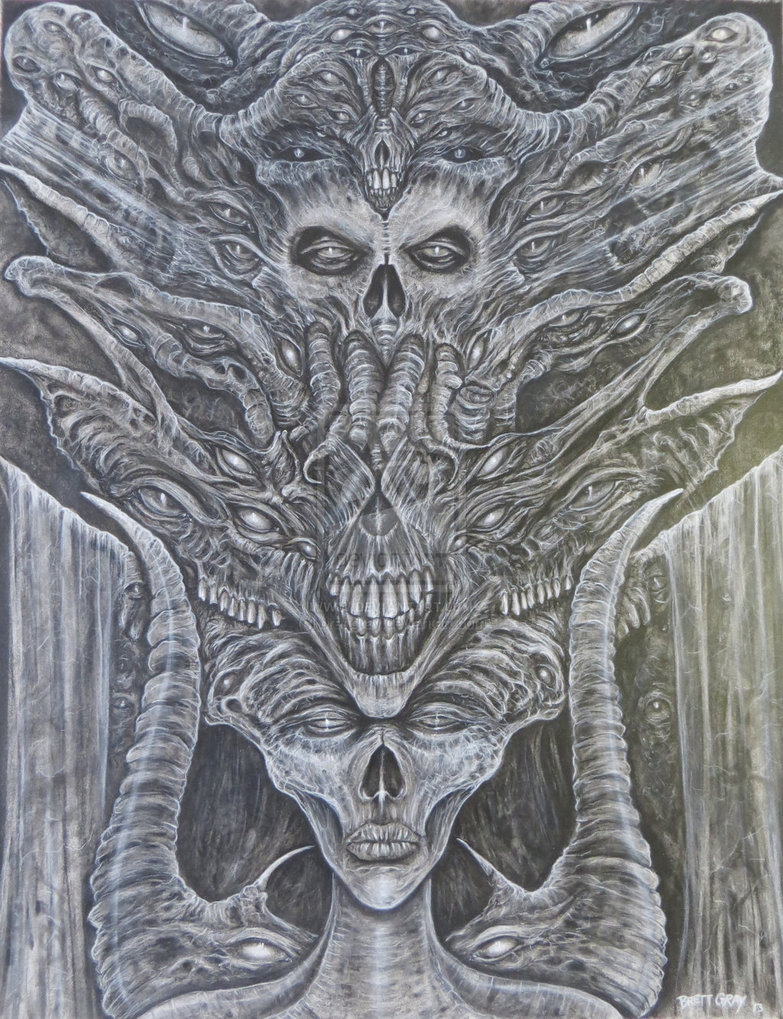
\includegraphics[scale=0.3]{priestess}
%\end{figure}
Birds chirp and the sounds of a flute hum in the atmosphere. The party comprises of Maden Rak, Exeter and Victoria. They travel through the Violet Forest to the Town of Bodmin. 

``Do you hear that?'' 

``I smell Elf.''

On a tree sits an Elf playing a flute. He is fully donned in black and brown leather armour. Over his face is a bandana. His pointed ears stand out prominently. 

``That is...'' before being interrupted by the Elf.

``Maden Rak. Special Forces Commander of the Midgaardian Roaches. Servant of the Dark. Hunter of Elves, murderer of women and children. Twice decorated for valour on the field of battle.'' He claps.

``Caeryn, son of a whore.''

``I've long awaited our meeting. Laid plans, set traps... And now you appear in my forest of your own volition.''

``We are here to bring to justice the Kingslayer and those who aid him. You will rot in a Midgaardian jail!''

``Good luck. This is our land. You will not win here.''

``Since when did the Elves hire professional killers to do their dirty work. The Elves have fallen low.''

``King or beggar, whats the difference? One Human less.''

``Dont make a big deal of the race thing.''

``Yet race is the very reason we fight! We have pointed ears, you have rounded. We have long lives, you have short. Yet you multiply quickly, like vermin, but die just as easily.''

``This is not about race, or freedom, or vengeance. You just refuse to see the obvious truth.''

``And what is that obvious truth?''

``That you are just being used by others.''

``That was a thing of the past! We shall not be used again.''

``Enough of this piss!'' Maden Rak throws a knife at the Elf, who then dodges clumsily in surprise, regains his footage, and then runs up to higher ground using the cover of archers. 
\normalfont

\newpage
\begin{multicols}{2}
This chapter goes through the process of creating a character in the world of Haeckel. There three ways of making characters. 

The basic method that is faster but has reduced options. I chose to build this system so that GMs could use it to help people quickly make characters on the fly such as when GMing in real life with a new gaming group. In this situation you often dont have the time to spend an hour (or more) on character creation.

It makes a party of Humans that are relatively skilled - being of the 1st level.   

And the advanced method which takes abit longer (and involves some reading) but more options. 

Characters built using either system are pretty much the same power level so the only key factor when choosing which to use is how much time you wish to spend making your character. 

The final system is the 0th level system. It makes a party of characters that are trained in a profession but not in adventuring. This system is for relatively mundane characters to be thrown in over their heads in some dire situation, as the GM requires. 

\section{Basic System 1st Level}

\begin{enumerate}
    \item The ability scores are: Strength (STR), Dexterity (DEX), Constitution (CON), Intelligence (INT), Wisdom (WIS), and Charisma (CHA). Record these down using the short hand version in brackets. 
    \item Roll 4d6 drop lowest for each ability score. Check the table below to see the 'ability score modifiers'. This number is based off your Ability Score and is the number that affects your dice rolls. 
    \item In the Basic System you default to a Human. Pick any Ability Score and increase it by +2.  
    \item Choose your class. Your options are: Fighter (STR), Wizard (INT), Rogue (DEX) and Cleric (WIS). Read the page on Core Classes. If you are a beginner player I highly suggest picking the Fighter class; however the Rogue and Cleric are okay for beginners too. I suggest only picking the Wizard class if you are an experienced player or want an additional challenge.
    \item Choose two ability scores to be Primary Attributes (this includes the bonus from being Human, as most other races would only get a choice of 1 Primary Attribute. Your class determines your third Primary Attribute. Your Primary Attributes represents the type of tasks you are best at solving while under pressure or with immense risk, and thus in a significant way shape the kind of character you have.
    \item Pick one equipment starting package. They are described below. Make a note of how much the package weighs. 
    \item You now need to calculate Carrying Capacity. This is equal to your Strength Ability Score. If Strength is your Primary Attribute you gain an additional +4. Likewise, if Constitution is one of your Primary Attributes you gain an additional +4 (stacking with the Strength bonus). For example, a Character with 16 Strength, and has a Primary Attribute of Str AND Con would have a carrying capacity of 24 (16+4+4).
\end{enumerate}

\begin{tabular}{l | r}
    Ability Score & Ability Modifier \\
    \hline
    18 & +3 \\
    16-17 & +2 \\
    13-15 & +1 \\
    9-12 & 0 \\
    6-8 & -1 \\
    3-5 & -2 \\   
\end{tabular}

%\begin{tabular}{l | c | r }
%Fighter Archetypes & Package & Space \\
%\hline
%Swordsman & Blah & 0 \\
%Archer & Blah & 0 \\
%Pikeman & Blah & 0 \\
%Axewielder & Blah & 0 \\
%\end{tabular}
%
%\begin{tabular}{|p{1.5cm}|p{5cm}|p{1cm}|}
%Rogue Archetypes & Package & Space \\
%\hline
%Lovable Rogue & Blah & 0 \\
%Burgler & Blah & 0 \\
%\hline
%Thug & Blah & 0 \\
%\hline
%Explorer & Crossbow, case with 20 bolts, short sword, 2 throwing daggers, sturdy leather armor, tanned brown cloak, thick tunic and pants, leather belt, low boots, backpack, 2 large treasure sacks, 50' rope, tinderbox, lantern, small hammer, 12 iron spikes, 2 flasks of military oil, wineskin, 2 weeks’ iron rations, 3gp & 0 \\
%\hline
%\end{tabular}
%
%\begin{tabular}{l | c | r }
%Cleric Archetypes & Package & Space \\
%\hline
%Priest & Blah & 0 \\
%Crusader & Blah & 0 \\
%Inquisitor & Blah & 0 \\
%Witch Hunter & Blah & 0 \\
%\end{tabular}
%
%\begin{tabular}{l | c | r }
%Wizard Archetypes & Package & Space \\
%\hline
%Witch & Blah & 0 \\
%Scholar & Blah & 0 \\
%Hedge Mage & Blah & 0 \\
%Monk & Blah & 0 \\
%\end{tabular}

\section{Advanced System 1st level}

\begin{enumerate}
    \item The ability scores are: Strength, Dexterity, Constitution, Intelligence, Wisdom, and Charisma. 
    \item Roll 4d6 drop lowest for each ability score.
    \item Choose your race. This may affect your ability scores. 
    \item Choose your homeland, and background.
    \item Choose your class. You can pick from any of the Core Classes or Campaign Classes. Your MAX HP is determined by your class choice and current Constitution ability modifier.
    \item Pick one sphere as your primary sphere.
    \item Pick one feat. The flaws are for more experienced players who would like an additional challenge.
    \item Choose your equipment. For fast play choose a starting package.
    \item Optionally pick a deity to follow. 
    \item Optionally choose a Faction that you aspire to join. 
    \item Optionally choose an Important Character for your character to know about and may want to be involved with. 
\end{enumerate}


\section{0th Level}

\begin{enumerate}
    \item Roll 3d6 for each ability score: Strength, Dexterity, Constitution, Intelligence, Wisdom, and Charisma.
    \item Roll 1d4 for health points, and add your Constitution modifer, as seen in the table above.
    \item Roll on the profession table to randomly determine your profession. This also determines your starting items.
    \item Choose your race. 
    \item Choose 1 ability score to be your Primary Attribute. Or choose 2 ability scores if you are a Human. 
\end{enumerate}

The way this works is basically: if a character survives the first adventure, they become a 1st level character. They may choose a class as per the usual rules. The weapon they used most during the adventure is the weapon they are proficient with at 1st level - unless they're a fighter, in which everything is proficient. 

\end{multicols}
